\chapter{Simulations}
\label{chap:method}

All simulations in this paper were performed using the \texttt{Janus} integrator \citep{2017arXiv170407715R} within the \texttt{Rebound} collisional N-body framework \citep{2012A&A...537A.128R}.

\section{Evolution of Earth-impacting cometary bodies in the inner Solar System}

%\subsection{Model Framework}

Our first numerical simulation involved a reverse-step integration examining the orbital migration of Earth-impacting cometary bodies in the Solar System.
The purpose of this was to generate simulation information on the orbital history of the cometary bodies, back from their Earth-impacting trajectories to points in their early dynamical lifetimes. This would help inform us on the nature of the cometary bodies' dynamical lifetimes and the various transfer mechanisms responsible for transporting them into the inner Solar System towards Earth. The framework for our simulation model is as follows:

We first include the Sun and all 8 planets of the Solar System - with the exclusion of their natural satellites. This was a decision taken to minimise computation time, as the short orbital periods of the natural satellites would have placed constraints on the integration time-step of our simulation. The gravitational effects of the natural satellites were assumed to have a negligible effect on the test particles throughout the course of the integration. Furthermore, there was a low prospect for collisions or encounters between test particles migrating through the Solar System and these natural satellites, due to their relatively low mass and sizes in comparison to the planets.

However, the assumption described does not hold true for the Moon - which plays an important role in Earth's dynamics. Due to the nature of this simulation involving Earth-impacting bodies, the effect of the Moon needed to be modelled appropriately. We therefore employed Newton's shell model to approximate the Earth-Moon system as a sphere of total radius $4\times10^5$ km, of combined mass $m_{earth}+m_{moon}$, with the centre of this sphere positioned at the centre of mass of the Earth-Moon system, orbiting in place of the Earth. This shell model consideration was able to improve computation times, by eliminating the need for short integration time steps that reflect the Moon's short orbital period in comparison to the planets.

\subsection{Initial Conditions}

We parametrised the initial conditions of the Solar System at the present epoch by describing the positions in space of all objects in our simulation with cartesian coordinates $(x,y,z)$, and velocity components $(v_x, v_y, v_z)$. Our values for position and velocity were taken to be the state of the Solar System at 01-01-2018 12:00 UTC - given by data sourced from the NASA JPL Horizons database\footnote{https://ssd.jpl.nasa.gov/horizons.cgi}.

We initialised the positions of Earth-impacting bodies by generating an isotropically distributed population of test particles on the surface of the Earth-Moon system. The test particles were chosen to be massless and collision-less -  this was due to the negligible masses of asteroids and comets in comparison to the larger planets, and the low probability of a collision between a small body and a planet. The choice for these test particles has the additional benefit of leading to a reduction in computation times.

Due to the extraordinarily sensitive starting conditions for N-body simulations of this nature, a Monte Carlo approach was adopted to generate $10^4$ test particles in an isotropic distribution. By randomly selecting initial orbital configurations for each test particle, the same overall final simulation result of the whole ensemble within a certain statistical tolerance could be rediscovered in repeat simulations.

\cite{shoemaker1962interpretation} has shown that for a gravitating body, the most probable impact angle is 45$^\circ$. Additionally, most studies involving planetary cratering rates assume that there is no spatial variation in meteor impact flux, and that the impact velocity and impact angle distributions are independent of position. Because of this, and due to the nature of the isotropic source of LPCs, we initialise our simulation so that there is an isotropic distribution of comets in a sphere around the Earth-Moon system.

We generate the initial $(x,y,z)$, coordinates for each test particle, by selecting values for the polar angle $\theta$ and azimuthal angle $\phi$ subject to the constraints,

\begin{equation}
  \begin{gathered}
    \theta = \cos^{-1}(2u-1); \; 0 \leq u \leq 1~, \\
    0 \leq \phi \leq 2\pi~,
\end{gathered}  
\end{equation}

where $u$ and $\phi$ are randomly and uniformly selected from within the stated ranges. We then transform to cartesian coordinates using,

\begin{equation}
\begin{split}
    x &= R\sin{\theta}\cos{\phi}~, \\
    y &= R\sin{\theta}\sin{\phi}~, \\
    z &= R\cos{\theta}~.
\end{split}
\end{equation}

where $R$ is taken to be $4\times10^5$ km (the radius of the Earth-Moon system). 

\subsection{Velocity Distribution}

%USE https://arxiv.org/pdf/1802.05034.pdf WHEN DESCRIBING VELOCITY DISTRIBUTION PEAKS

Numerous meteoroid velocity distributions have been derived from observations (eg. \citep{HUNT200434} with the use of high-gain radar). However these distributions are made up of poor cometary statistics and are liable to underestimations in the number of high velocity, fragmentation-prone meteoroids.

Because of this, we generated a synthetic velocity distribution for Earth-impacting LPCs. This was modelled using a Monte Carlo simulation, assuming an isotropic parabolic source distribution. Using the method described by \cite{2000MNRAS.315..629H}, assuming that the Earth is moving at a constant velocity in a circular orbit, the expected comet-Earth collision velocities $V_i$ were extracted from this synthetic population of comets using,

\begin{equation}
    V_i^2 = \sqrt{\dfrac{2GM_\Earth}{R_\Earth}} + GM_\odot \left(\dfrac{3}{r_\Earth}-2 \sqrt{\dfrac{p}{r_c^3}} \cos i - \dfrac{1}{a}\right) ~,
    \label{eq:im_vel}
\end{equation}

where $M_\Earth$ and $M_\odot$ are the masses of the Earth and Sun respectively, and $r_\Earth$ and $r_c$ are the radii of the Earth's and comet's orbits respectively ($r_\Earth = 1$ AU). $p$, $a$ and $i$ are the semi-latus rectum, semi-major axis, and inclination elements of the comet's orbit respectively, and $R_\Earth$ is the radius of the Earth. The gravitational influence of the Moon on incoming meteoroids was taken to be negligible in comparison to the Earth - so no additional considerations were taken for the generated Earth-impact velocities prior to launching test particles from the surface of the Earth-Moon system.

\begin{figure}[t!]
    \centering
    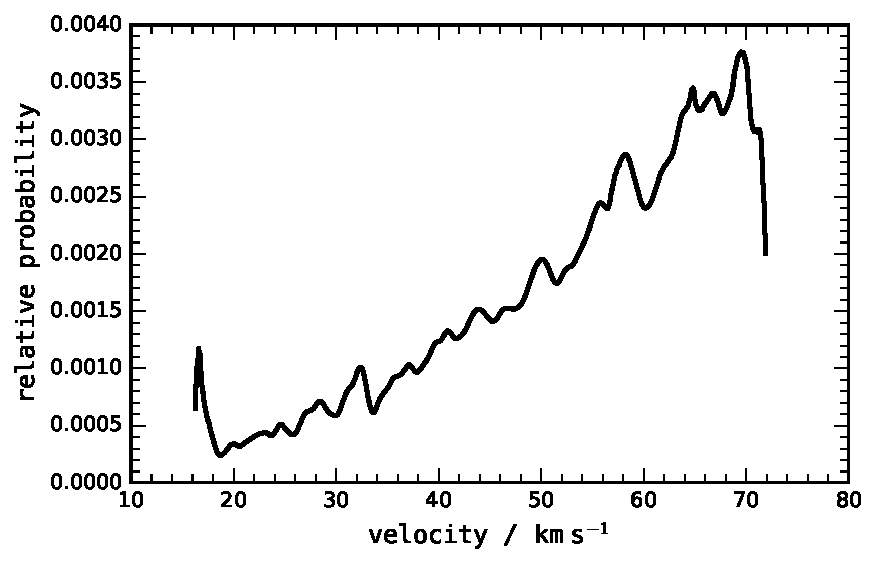
\includegraphics{vel_dist.pdf}
    \caption[Velocity distribution of Earth-impacting cometary meteoroids]{Synthetic impact velocity distribution of LPC meteoroids at the Earth.}
    \label{fig:vel_dis}
\end{figure}

Fig.~\ref{fig:vel_dis} shows the synthetic Earth impact velocity distribution for LPCs. We see that the plot exhibits a peak at both ends of the distribution. These represent the two different extremes of a comet-Earth impact - where a comet is orbiting on the same plane as the Earth and collides on either a prograde or retrograde approach. 

The mean impact velocity is 54 km$\;$s$^{-1}$, in agreement with 53 km$\;$s$^{-1}$ reported by \cite{1988merc.book..274S} for LPC impacts. The calculated distribution was therefore accepted as an appropriate characterisation of impacting comets' velocities for use in the simulation.

By considering an Earth-impacting comet, with aphelion very far from the Sun, one can use the escape velocity $v_{esc}$ of the Sun for the comet orbiting on the plane of the ecliptic at 1 AU. Using $v_{esc}=\sqrt{2GM_{\odot}/r}$ where $M_{\odot}$ is the mass of the Sun and $r$ is the distance from the Sun to the comet, the maximum speed for a cometary body impacting the Earth is 42.2 km$\;$s$^{-1}$. This is the maximum velocity for an Earth-approaching comet - otherwise it would not be gravitationally bound to the Solar System. 

By considering a head-on Earth impact as well as an Earth-impact facing the planet behind its direction of travel, the minimum and maximum cometary impact velocities are given by,

\begin{equation}
    (\sqrt{2}-1) \sqrt{ \dfrac{GM_{\odot}}{1 AU} } \leq |v_i| \leq (\sqrt{2}+1) \sqrt{\dfrac{GM_{\odot}}{1 AU}} ~,
\end{equation}
 
 These bounds for a cometary meteoroid distribution support the synthetic result shown in Figure.~\ref{fig:vel_dis}.

%By considering the escape velocity $v_{esc}$ of the Sun for an object orbiting on the plane of the ecliptic at 1 AU, one can use $v_{esc}=\sqrt{2GM_{\odot}/r}$ where $M_{\odot}$ is the mass of the Sun and $r$ is the distance from the Sun to the comet, to calculate the minimum and maximum speeds for a cometary body impacting the Earth. By considering a head-on Earth impact as well as an Earth-impact facing the planet behind its direction of travel - an initial choice for the launch velocity $v$ of each test particle was then selected - such that in the reference frame of the Solar System, the condition $12.4$ km$\;$s$^{-1} \leq |v| \leq 71.9$ km$\;$s$^{-1}$ held true. The absolute minimum and maximum velocity of a cometary meteoroid represent cases where the comet resided on the plane of the ecliptic. This is an unlikely scenario as, for example, LPCs are isotropically distributed. Therefore further selections on velocities were required in order to adequately model the lower expectations for higher-velocity impacts in this range.

%We achieved this by fitting a curve to a meteoroid velocity distribution by \cite{HUNT200434}. This distribution was based on data from the Canadian Meteor Orbit Radar (CMOR) \citep{2014pim3.conf...84W}, which had a large sample size ($>$ 3000) of high velocity meteoroids, making the statistics more reliable for cometary meteoroids.

%The distribution was replicated by fitting two Gaussian distribution functions to the data from \cite{HUNT200434} (See Figure.~\ref{fig:vel_dis}). In order to replicate the distribution, the first Gaussian fit was used for the range 17 km$\;$s$^{-1}$ to 48 km$\;$s$^{-1}$ and the second Gaussian fit was used in the range 48 km$\;$s$^{-1}$ to 72 km$\;$s$^{-1}$.

%The requirement for two curves needing to be fit to the distribution was assumed to be indicative of asteroid and cometary meteoroids. Due to the difficulties in extracting the cometary velocity distribution alone - the velocity distribution representative of all asteroidal and cometary meteoroids was chosen. A filtering mechanism was then employed at the conclusion of the simulation based on dynamical characteristics, in order to extract the cometary population alone (detailed in \S~\ref{chap:results}). For each particle, the velocity of the Earth-Moon system was summed onto a velocity sampled from this replicated distribution.

For each test particle in the simulation, an initial choice of velocity was randomly selected from the generated distribution. Additional final considerations were then applied to the selected velocities. Due to the nature of the random sampling of velocities and positions it was, for example, entirely possibly for a test particle to be assigned a position on the surface of the Earth-Moon system with a velocity vector that caused it to fall towards the Earth upon a reverse-step integration. As this is not the intended behaviour for this simulation of Earth-impacting comets, additional checks were required. If the velocity vector was directed inside the Earth-Moon system, the test particle's location and velocity was reselected. Additionally, if the magnitude of the velocity vector (when summed to the velocity of the Earth-Moon system) exceeded 72 km$\;$s$^{-1}$, the velocity vector was rejected and a new one selected.

\subsection{Launching Routine}

In order to replicate impactors arriving at Earth at different time periods, the population of test particles were gradually released over a time period of 12 yrs. The time period for launches was determined by a random generator using a normal distribution.  The reason for this decision was because Jupiter plays one of the most important roles in influencing the orbits of small bodies in the Solar System - and releasing the test particles over a time period similar to the orbital period of Jupiter was an important decision to help replicate the various different gravitational interactions small bodies have with Jupiter at different points in its orbit.

The Solar System is chaotic, with a Lyapunov timescale of $\sim 5$ Myr \citep{1996CeMDA..64..115L}. A time period of 10 Myr was chosen to be the length of the simulation, in order to fully capture a period of Solar System stability. The integration routine ran with a reverse time step of -6 days, with data snapshots taken every 500 years. At each snapshot the orbital parameters of each simulated body were recorded and written to a .hdf5 file for later analysis. The length of our integration was chosen such that there was not an unnecessarily large expenditure of computing resources, while physically meaningful results were still produced.

\section{Simulating Earth observations of an impending comet impact}

\begin{equation}
    m = H + 5\log(r_{hel}r_{geo}) - 2.5\log(\phi(\theta))~.
\end{equation}




\iffalse

\subsection{Generating a synthetic population of hazardous long-period comets}

We first generate a synthetic population of hazardous long-period comets, by creating a population of comets subject the following orbital constraints on semi-major axis $a$, inclination $i$ and perihelion distance $r_p$,

\begin{equation}
    \begin{gathered}
        2000 \text{ AU} \leq a \leq 100,000 \text{ AU}~,\\
        0^{\circ} \leq i \leq 180^{\circ}~\\\
        6 R_\odot \leq r_p \leq 1 \text{ AU}~.
    \end{gathered}
\end{equation}

The resulting orbits were then modified further so that they become Earth-impacting. This is carried out by first finding a value of $\theta$ such that $f(\theta)$ is minimised where,

\begin{equation}
    f(\theta) = | \; r_{\Earth} - ||\vec{r}(M = \theta, \omega = 0, a, e, i, \Omega)|| \; | ~,
\end{equation}

and,

\begin{equation}
   r_{\Earth} = ||\vec{r}(M_{\Earth}=\Omega, \omega_{\Earth}, a_{\Earth}, e_{\Earth}, i_{\Earth}, \Omega_{\Earth})||~,
\end{equation}

where $r$ is the distance between the object and the Sun.

A value for $\phi$ is then found such that $f(\phi)$ is minimised where,

\begin{equation}
    g(\phi) = | \; \vec{r}(M = \theta, \omega = \phi, a, e, i, \Omega) \cdot \vec{z} \; | ~,
\end{equation}

where $\vec{z}$ is the Earth's orbital normal vector.

A random lead time $t_l$ is then found, subject to constraints. The comet's and Earth mean anomalies are set to $M = \theta^{\prime}$ and $M_{\Earth} = \theta^{\prime}_{\Earth}$ respectively,

\begin{equation}
    \begin{split}
        \theta^{\prime}_{\Earth} &= \Omega - \dfrac{t_l \sqrt{GM_\odot}}{2\pi {a_{\Earth}}^{3/2}}~, \\
        \theta^{\prime} &= \theta - \dfrac{t_l \sqrt{GM_\odot}}{2\pi {a_{a}}^{3/2}}~.
    \end{split}
\end{equation}

where $M_\odot$ is the mass of the Sun.

\fi